\documentclass[a4paper,titlepaget]{article}
\usepackage[T1]{fontenc}
\usepackage[utf8]{inputenc}
\usepackage[english]{babel}
\usepackage{amsmath}
\usepackage{graphicx}
\usepackage{graphics}
\usepackage{caption}
\usepackage{amssymb}
\usepackage{listings}
%\textwidth=450pt\oddsidemargin=0pt
\date{9 July 2020}

\begin{document}
\title{\textbf{Report of Final Project:\\ Tree Localization by semantic superpixels classification}}
\author{Luca Dolci, 1234008}
\maketitle
\newpage


\section{Task presentation and my approach}
This project aim to localize trees in an image, by drawing a bounding box
around them. Lots of different approaches can be use. Fully aware that the best
one is maybe use a well trained CNN with image pyramid and sliding windows, my
approach is different, in the sense that I decide to not use any NN-based
classifier.

\subsection{High level description of my approach}
My approach is based on SVM classification on quantized SIFT
descriptors in a superpixel segmented image, in a BOW-fashioned way, followed by merging in order to localize an entire tree. My approach
is basically an implementation of \emph{Class Segmentation and Object Localization with Superpixel Neighborhoods} by Brian Fulkerson, Andrea Vedaldi and Stefano Soatto\footnote{https://ieeexplore.ieee.org/document/5459175} coupled with some ideas taken from different papers and some original ideas.

\noindent Workflow:
\begin{enumerate}
	\item Superpixel segmentation: a superpixel is an area in the image with some spatial, color and texture consistency. A superpixel sementation is the task to divide the image in non-overlapping superpixels.
	\begin{figure}[htpb]
		\centering
		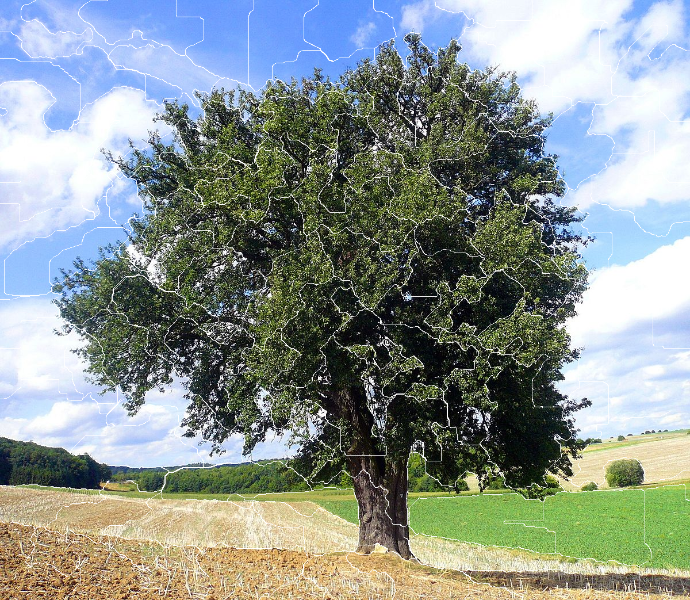
\includegraphics[width=.6\textwidth]{images/superpixel_segmentation}
		\caption{\centering An example of a 100-superpixel segmentation done by
        SEEDS algorithm.}
	\end{figure}
	\item Features extraction: SIFT features are extracted for each superpixels
        in previous step.
	\item SIFT quantization: the SIFT descriptors are quantized using Bag Of Words to obtain a
        single, aggregated, descriptor.
    \item Histogram Agglomeration (optional): the descritors of neighborhoods superpixel are aggregated
        to perform a better classification.
    \item Classification: superpixel are classified using a binary SVM trained on aggregated
        descriptors to obtain a prediction map
	\begin{figure}[htpb]
		\centering
		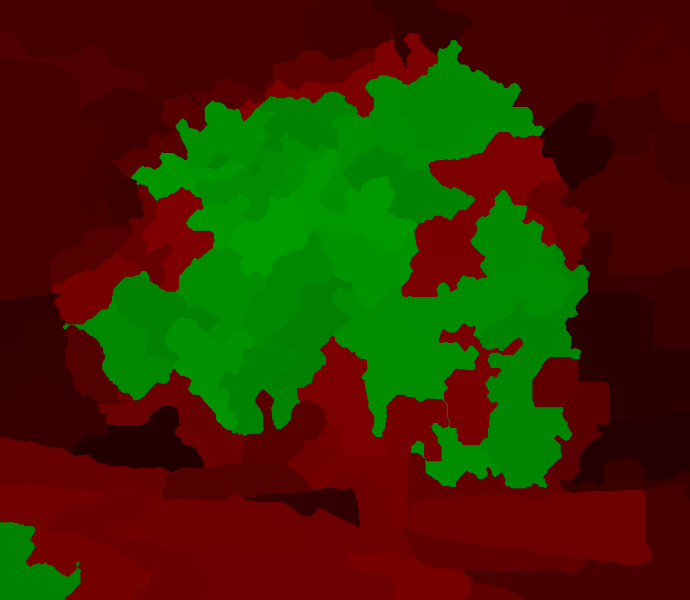
\includegraphics[width=.6\textwidth]{images/prediction_map}
		\caption{\centering The prediction map for each superpixel, red  mean
        negative response, green means positive response.}
	\end{figure}
    \item CRF refinement (optional): the result can be refined using a Conditional Random Field
        to obtain better boundaries
    \item Merging: positive response superpixels are merged in order to localize
        the trees
	\begin{figure}[htpb]
		\centering
		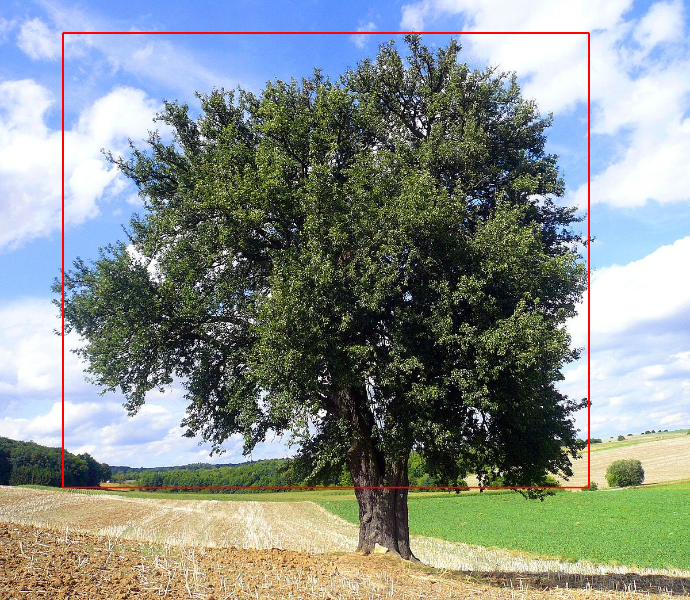
\includegraphics[width=.6\textwidth]{images/result}
        \caption{\centering Final result.}
	\end{figure}
\end{enumerate}


\subsection{Implementation and design choices}
\subsubsection{Superpixel Segmentation}
Despite that in the original paper \emph{quickshift} superpixel segmentation algorithm is used, I decided to use the \emph{SEEDS} algorithm among the three possible choices of segmentation algorithms implemented in OpenCV (the other two are \emph{LCS} and \emph{SLIC}). I used \emph{SEEDS} for two reasons: it's fast and it can easily control the number of superpixels to create. In fact, despite that the other two (especially \emph{SLIC}) produces better results (in terms of accuracy in borders), it is not possible to specify the number of superpixels, but instead, a region size, which is not so easily controllable, even with rescaling and other tricks.

The number of superpixels $N_{superpixels}$ is set between 200 and 2000 and in general is a design parameter. Usually 750 is selected. In the original paper, this number is higher (around 2000) but to maintain feasible the next computations, this number is maintained low, also to permit a more uniform feature density among superpixels (small superpixel has low chance to contain features, so there's no a strong confidence on the future classification). An high value can lead to a coarse classification, a small one can bring to a small and unjoined areas that covers partially the tree.

Before segmentation, a gaussian blur and a conversion on CIELab color space are performed in order to increment performances. In this step connectivity, color, centers and other proprierties are computed.

This step takes no more than 1000ms, but can be tuned to 500ms.

\subsubsection{Feature Extraction}
SIFT features with descriptors are extracted from the image. No parameter tuning is done in this step, so the features are extracted as usual and not in a very dense way like the original paper. I tried also the last possibility but the results were not satisfactory. 

There's a big drawback in this step: no features are extracted in a very low light condition, so a very dark-illuminated tree is not correctly classified due to few features. Also, the choice of segmentation algorithm has to be precise in the sense that the extrema part of a tree (composed by few leaves) has to be thin in the sense that it is a high feature density region and if it is too wide it can cause false positive. \emph{SEEDS} is chosen also because it avoids these situations.
\begin{figure}[htpb] 
	\centering
	\begin{minipage}{.3\textwidth}
		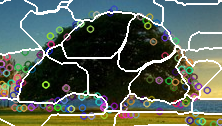
\includegraphics[width=1.2\textwidth]{images/black_tree} 
	\end{minipage}
	\hspace{.15\textwidth}
	\begin{minipage}{.3\textwidth}
		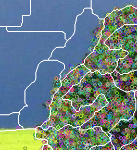
\includegraphics[width=\textwidth]{images/leaves}
	\end{minipage}  
	\caption{\centering Problems with features: no feature are extracted in black areas (left) and leaves superpixel has to be thin because of lots of features (right)}
\end{figure}

\subsubsection{SIFT quantization}
SIFT features are quantized using Bag Of Words trained with photos segmented with 150 superpixels. Then $k$-means is performed with $k$=400, to have a good variability in the possible descriptors. 
After training, the descriptors' histograms are quantized using this trained BOW, so for each superpixel, a 400-dimensional vector/histogram will be computed. Each entry of this vector represents the ($l_1$ normalized) frequency of encountering a feature in the superpixel which is also in the vocabulary. This histogram will be the input of the classifier

400 is chosen but a higher value can be used. I tried also with 1000 and more clusters but the results are similar, so I left this parameter as 400.

\subsubsection{Histogram Aggregation}
For a single superpixel, it's histogram is aggregated and $l_1$ normalized with the $N$ closest superpixels (usually a value between 0 and 4). The distance can be computed in various ways like the cityblock distance between center or the distance between color in various color spaces. In my implementation, I used a mixed approach: the first front of BFS is computed, then I select the first $N$ closest superpixel by $l_2$ disatnce on HSV color space: this helps to preserve boundaries of the trees because SEEDS tends to form superpixel with crazy shape (not rectangular-like, as \emph{SLIC} or \emph{LSC}). 
This process helps the classifier in two ways: as a form of regularization and as an improvement of the BOW because the 400 bins histogram is very sparse, caused by the high dimensionality.

\subsubsection{SVM classification}
A binary SVM is trained on 250 pre-segmented photos, both with trees and grass (ADE20k dataset). A superpixel is considered $\in \ TREE$ class if at least 95\% of its pixels are segmented as a tree. A $\chi^2$ kernel is used. $C$, the regularization parameter as $\gamma$ are picked with $k$-fold cross-validation. 

The implementation is done on OpenCV SVM, and this is the main drawback of the project. The best training error achieved is around 15\%, which is very high and is the main reason for the generally poor results. I tried lots of different configurations, like different kernels, any form of histogram equalization in different color spaces, any combination of parameters but with the tools in my posses (a 6-yo old laptop) I really couldn't train a good SVM. I also tried to convert the code to python and run it on Google Colab, with no success (training time was the same, taking apart Colab crashes). In a future implementation, I really want to try the \texttt{libsvm} library which will necessarily be better. 

Another drawback of OpenCV implementation is that the output is not well defined. In fact, taking apart a flat +1/-1, it is only possible to have the inner product between the sample and the vector defined by support ($\underline{w}\cdot\underline{h}+b$ in ML notation), a very raw result (also this part is not so well documented), which is a value in range $(-\infty..1]$ and not 0-centered. OpenCV implementation applies a sign to this result in order to have the class label, but I applied a sigmoid instead. The sigmoid can be tuned independently on the right and on the left part, in order to have a 0-1 probability with some confidence.

This step takes around 250ms for all superpixels.

\subsubsection{Random Field refinement}
The labels computed previously acts as a node potential $\psi$ for a CRF while the edge potential is defined as follows:
\begin{equation*}
	\phi = \frac{L(s_i,s_j)}{1+||s_i - s_j||}
\end{equation*}
where $L$ is the lenght of the common border between superpixel $s_i$ and $s_j$ and $||s_i - s_j||$ is the $l_2$ norm of color difference in the LUV colorspace. We have both spatial and color consistency. A tradeoff between $\phi$ and $\psi$ is applied.

This step is not strictly necessary since we perform superpixel segmentation with lots less superpixel than the one performed in the original paper. Anyway, even with few superpixels, the result can improve a bit, in the sense that some single-superpixel object false positive are suppressed, but the results are comparable. 

This step takes no more than 500ms.

\subsubsection{Superpixel merging}
The positive-response superpixels are merged in order to localize the tree. The merging process is simply done on connectivity. Too small component (composed by a few superpixels) are discarder. No future discard are performed.

\subsection{How to improve results}
The results can be improven by simply train a better SVM. A chain is strong as it's weakest link, and SVM is the weakest link. With a robust classifier the entire workflow will became automatic, in the sense that there's no a parameter to tune. But this is not the case, in fact, in the results I'm going to present in the next section, $N_{superpixel}$ and $N$ will change also to show the difference and the behaviour of the approach under that changes. $N_{superpixel}$ is simply a threhsold between false positive rate and better boudaries and $N$ is a connectivity helper.

I could easily couple this type of classification with some threshold on green in HSV color space, clustering on colors, factal dimension computation for boudaries and many more to fix the issues with SVM but I'm not going to do it. In my opinion it's better to fix a broken thing instead of finding workarounds. The next results will be considered as raw, due to a not well trained SVM on inadeguated tools. (the very first three images are an example: they are obtained with a different SVM and the results are better)

\newpage
\section{Results on test set}
\subsection{Result on test 1}
\begin{figure}[htpb] 
	\centering
	\begin{minipage}{.3\textwidth}
		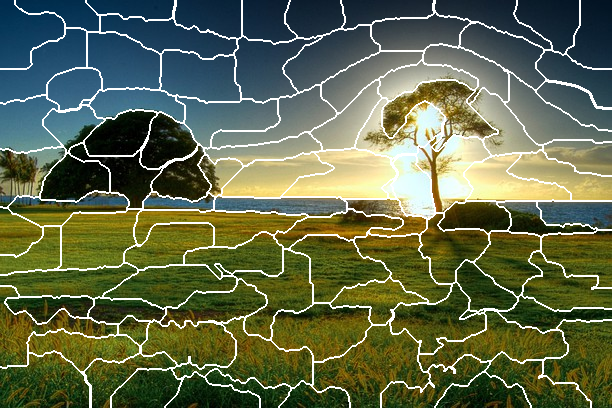
\includegraphics[width=1.7\textwidth]{images/results/1seg} 
	\end{minipage}
	\hspace{.25\textwidth}
	\begin{minipage}{.3\textwidth}
		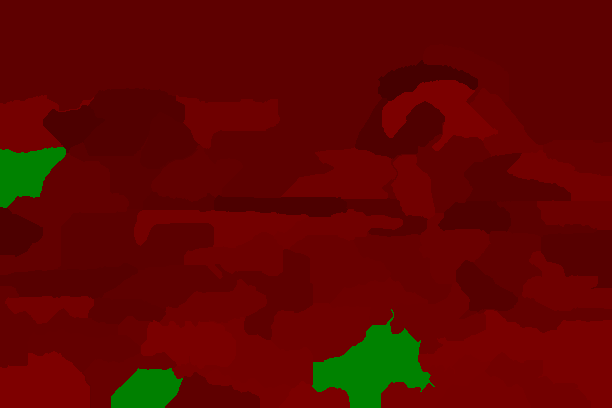
\includegraphics[width=1.7\textwidth]{images/results/1map}
	\end{minipage}  
\end{figure}
\begin{figure}[htpb]
	\centering
	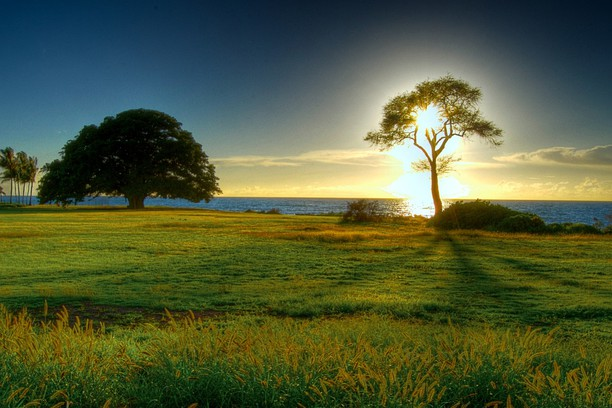
\includegraphics[width=.9\textwidth]{images/results/1fin}
\end{figure}
$N_{superpixel}=250$, $N=2$. Here we have no localization due to few features computed in both high and low illuminated areas. Notice that The small trees on the left are correctly classified but discarded due to dimension.
\newpage

\subsection{Result on test 2}
\begin{figure}[htpb] 
	\centering
	\begin{minipage}{.3\textwidth}
		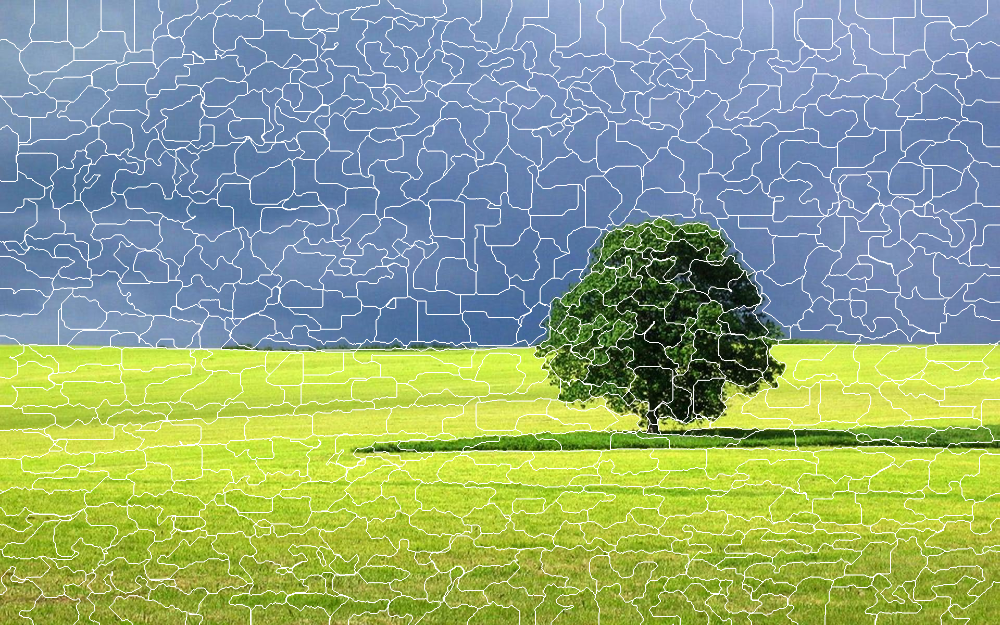
\includegraphics[width=1.7\textwidth]{images/results/2seg} 
	\end{minipage}
	\hspace{.25\textwidth}
	\begin{minipage}{.3\textwidth}
		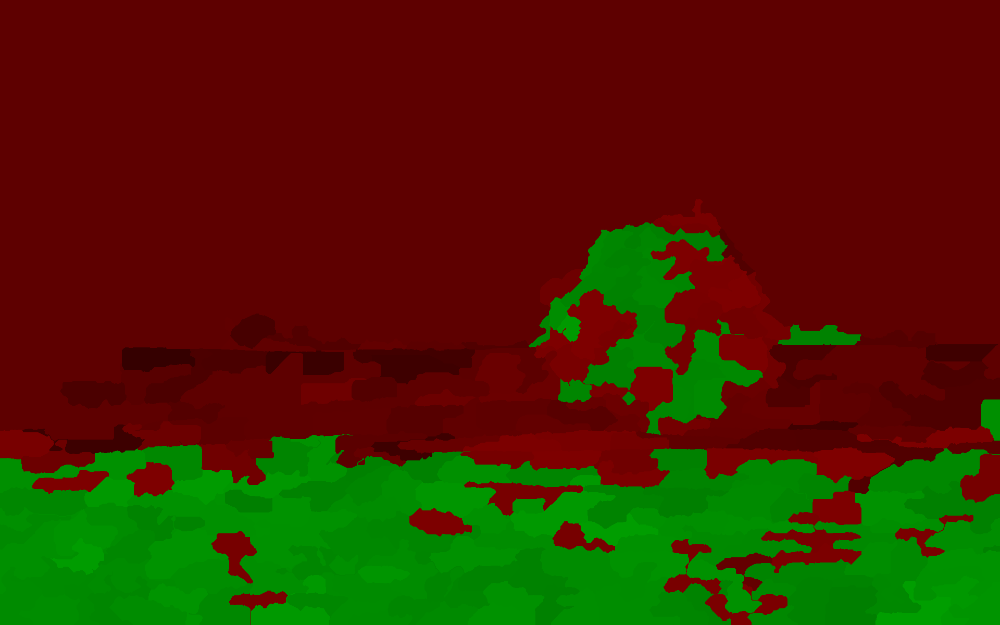
\includegraphics[width=1.7\textwidth]{images/results/2map}
	\end{minipage}  
\end{figure}
\begin{figure}[htpb]
	\centering
	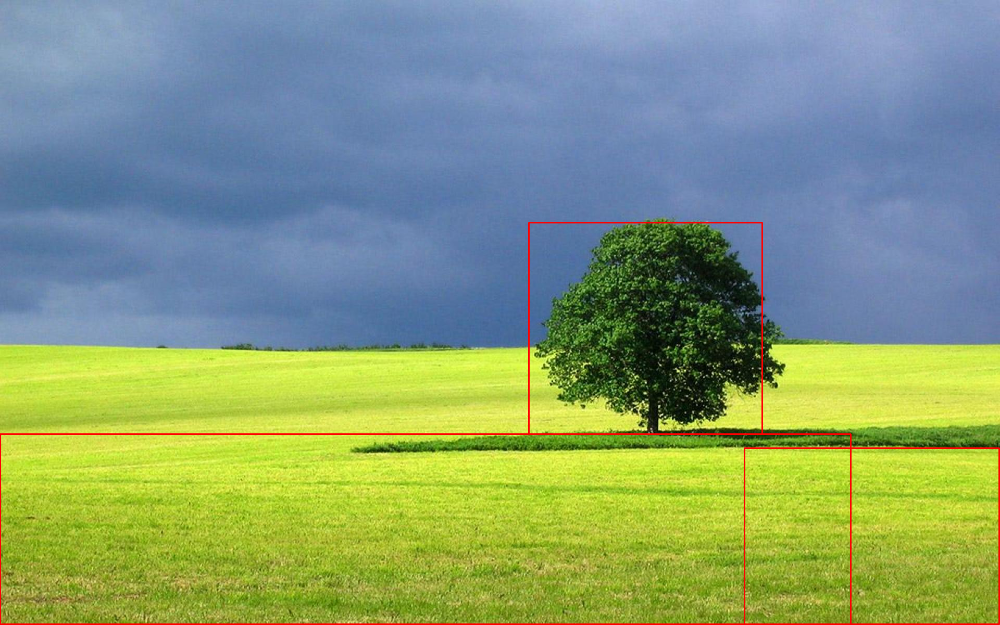
\includegraphics[width=.9\textwidth]{images/results/2fin}
\end{figure}
$N_{superpixel}=750$, $N=0$. The tree is nicely localized but we have two false positive that can be discarded by color thresholding. Notice that in the segmentation, darker area of the tree are enclosed in a superpixel and they are not classified correctly.
\newpage

\subsection{Result on test 3}
\begin{figure}[htpb] 
	\centering
	\begin{minipage}{.3\textwidth}
		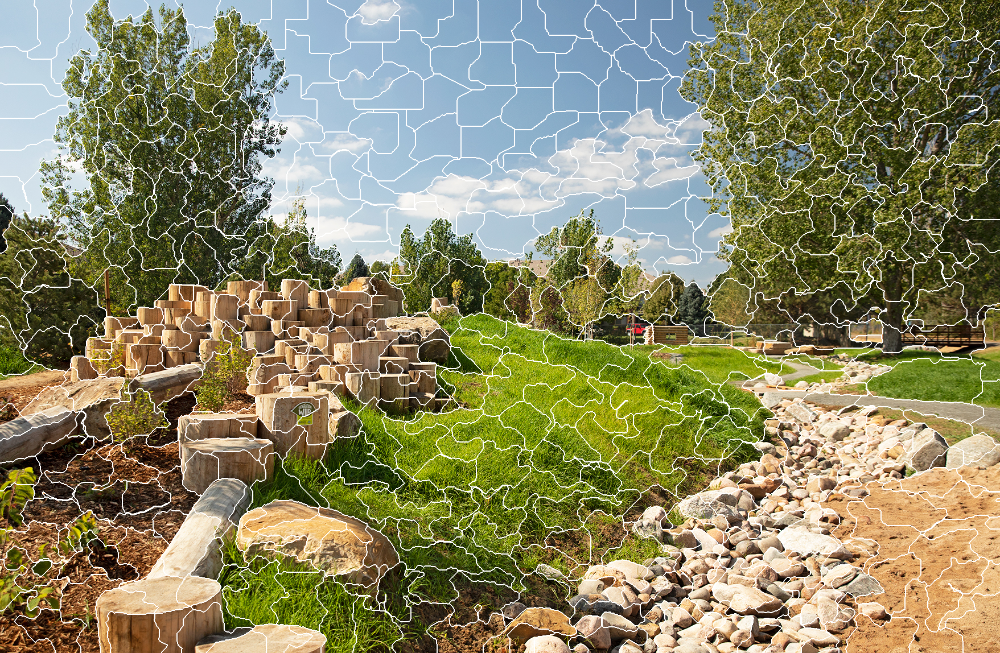
\includegraphics[width=1.7\textwidth]{images/results/3seg} 
	\end{minipage}
	\hspace{.25\textwidth}
	\begin{minipage}{.3\textwidth}
		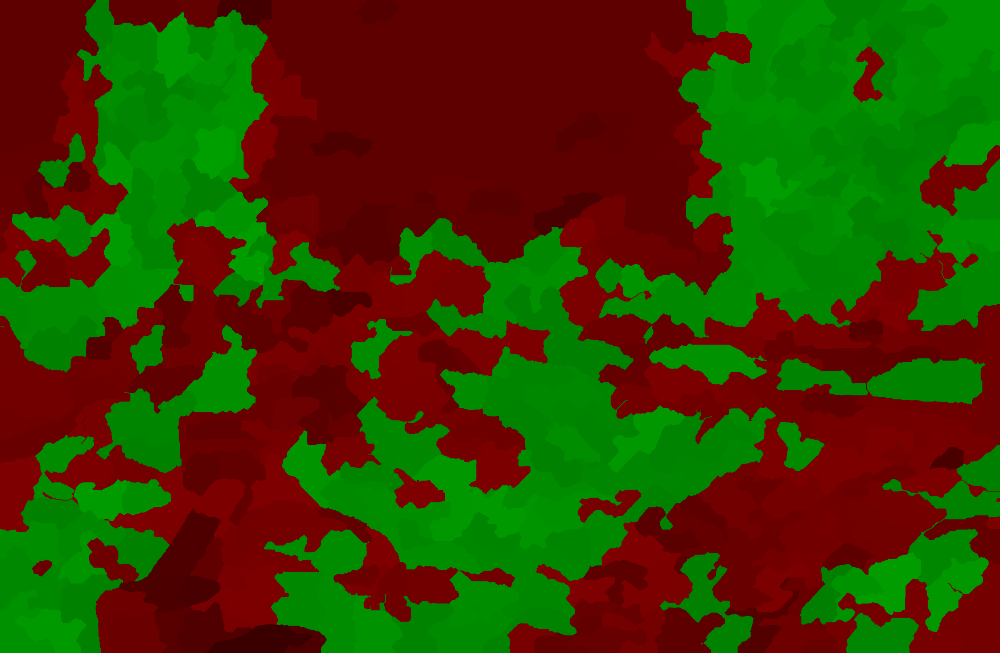
\includegraphics[width=1.7\textwidth]{images/results/3map}
	\end{minipage}  
\end{figure}
\begin{figure}[htpb]
	\centering
	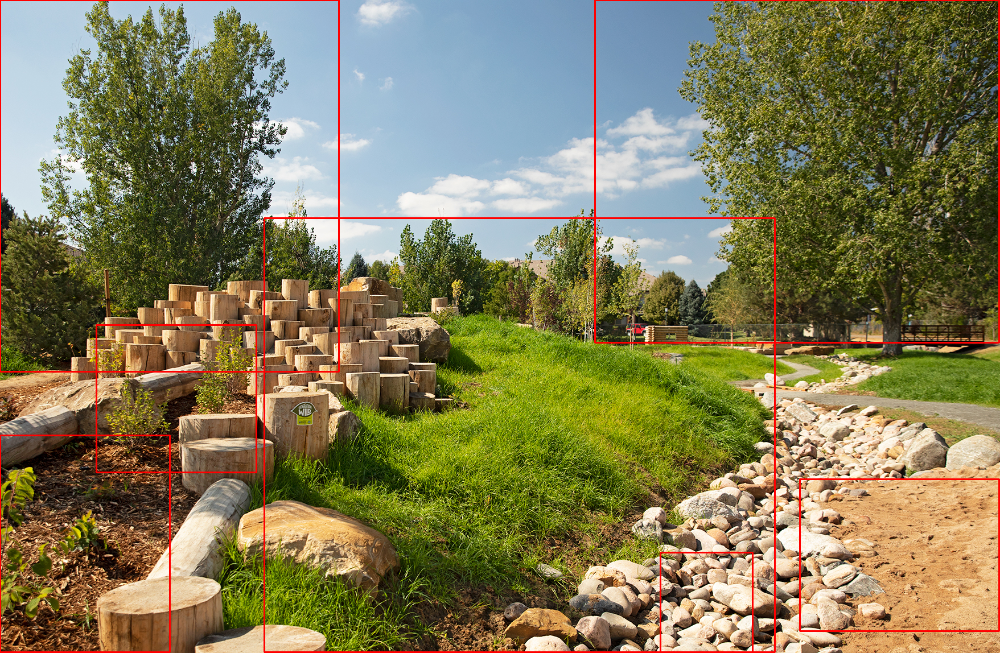
\includegraphics[width=.9\textwidth]{images/results/3fin}
\end{figure}
$N_{superpixel}=750$, $N=0$. The two main trees are correctly localized. The one on the right has a bigger bounding box due to an horizontal superpixel. There are two false positive that can be discarded by color thresholding, other two (on the left) corresponds to the small trees and the green leaves are missclassified and we have a central big bounding box corresponding to the green chunk in the middle. Clearly an error. If the resolution of the image is elevated, it's ok to increase $N_{superpixel}$, but we will have more false positive. The high presence of green suggest to use a lower $N$. 
\newpage

\subsection{Result on test 4}
\begin{figure}[htpb] 
	\centering
	\begin{minipage}{.3\textwidth}
		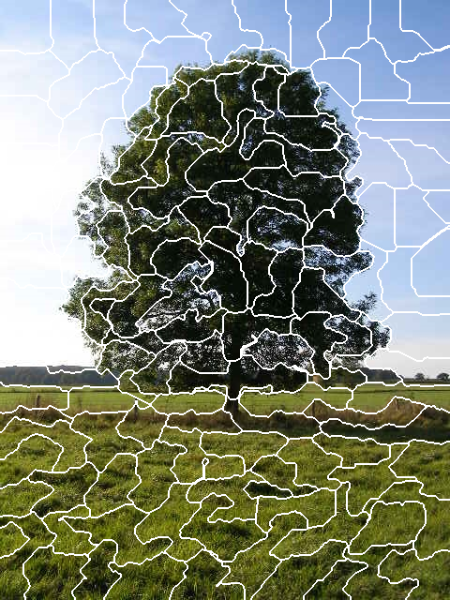
\includegraphics[width=1.2\textwidth]{images/results/4seg} 
	\end{minipage}
	\hspace{.15\textwidth}
	\begin{minipage}{.3\textwidth}
		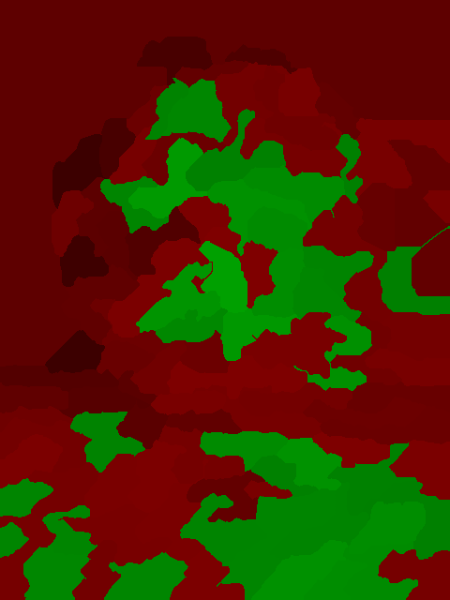
\includegraphics[width=1.2\textwidth]{images/results/4map}
	\end{minipage}  
\end{figure}
\begin{figure}[htpb]
	\centering
	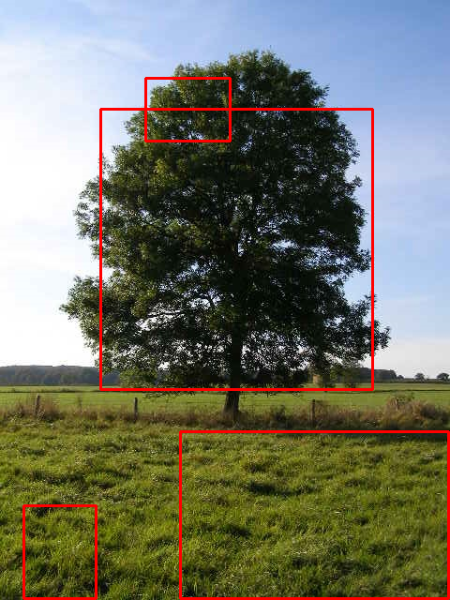
\includegraphics[width=.6\textwidth]{images/results/4fin}
\end{figure}
$N_{superpixel}=250$, $N=0$. The tree is not correctly localized, the top is outside the bouding box due to a superpixel that is not connected to the rest of the tree. There are also two false positive that can be discarded by a better classifier. Notice that, even if the SVM is trained on full tree, it's very difficult to include the trunk in the bouding box. 
\newpage

\subsection{Result on test 5}
\begin{figure}[htpb] 
	\centering
	\begin{minipage}{.3\textwidth}
		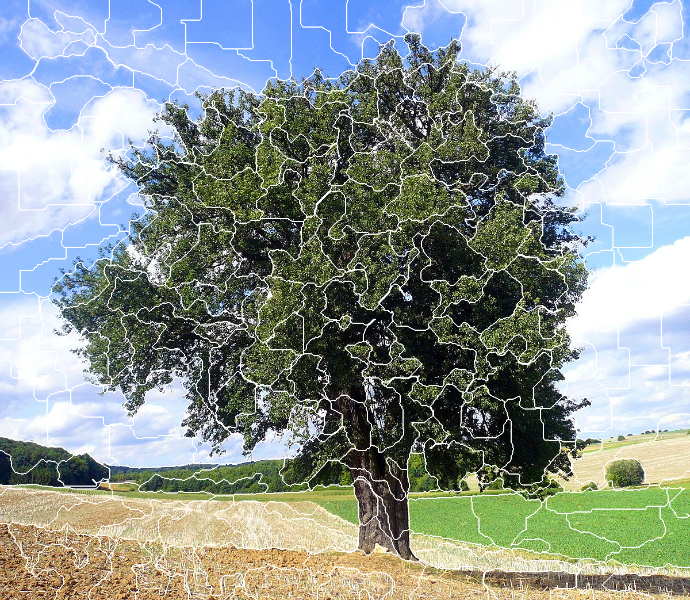
\includegraphics[width=1.7\textwidth]{images/results/5seg} 
	\end{minipage}
	\hspace{.25\textwidth}
	\begin{minipage}{.3\textwidth}
		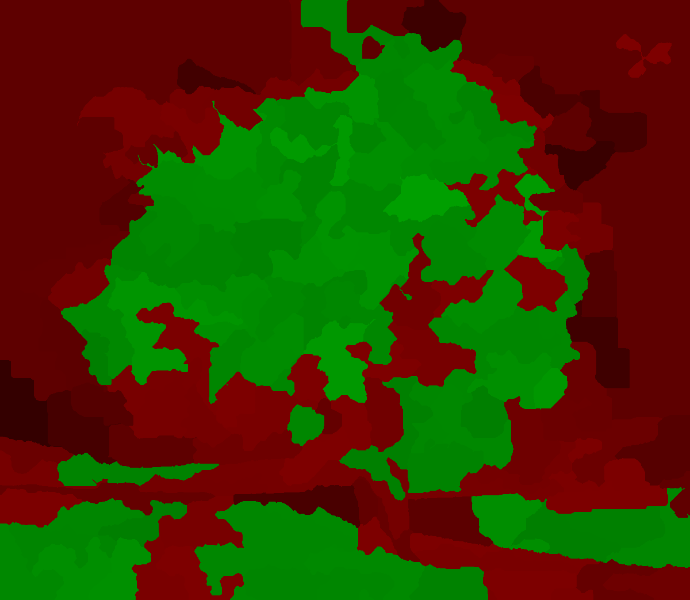
\includegraphics[width=1.7\textwidth]{images/results/5map}
	\end{minipage}  
\end{figure}
\begin{figure}[htpb]
	\centering
	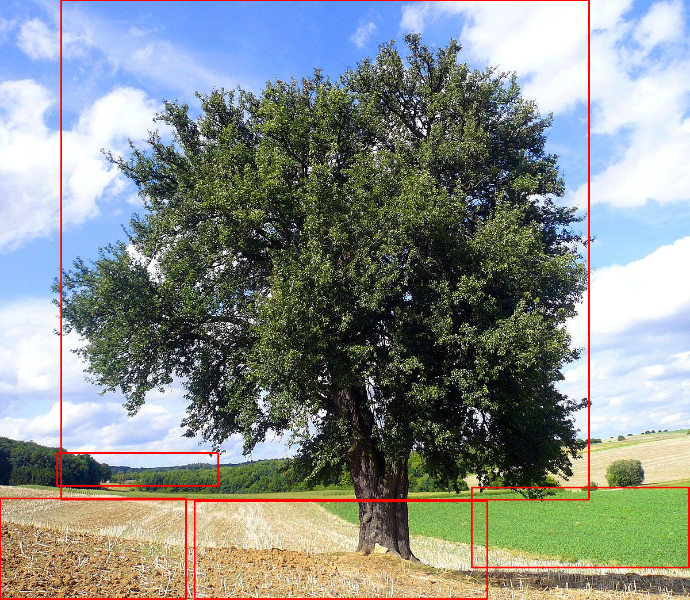
\includegraphics[width=.9\textwidth]{images/results/5fin}
\end{figure}
$N_{superpixel}=250$, $N=0$. The tree is not correctly localized, there's some sky that is inside the bouding box. The other trees can be discarded by color thresholding.
\newpage

\subsection{Result on test 6}
\begin{figure}[htpb] 
	\centering
	\begin{minipage}{.3\textwidth}
		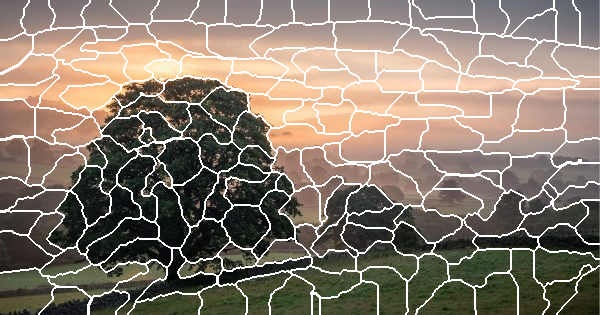
\includegraphics[width=1.7\textwidth]{images/results/6seg} 
	\end{minipage}
	\hspace{.25\textwidth}
	\begin{minipage}{.3\textwidth}
		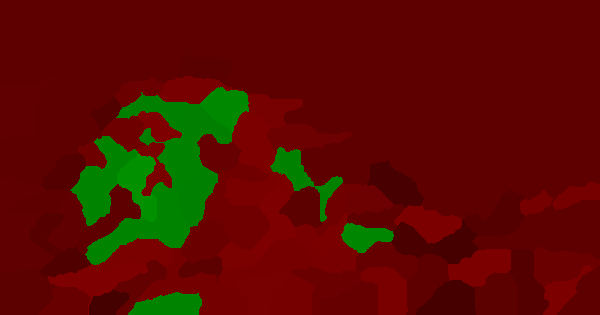
\includegraphics[width=1.7\textwidth]{images/results/6map}
	\end{minipage}  
\end{figure}
\begin{figure}[htpb]
	\centering
	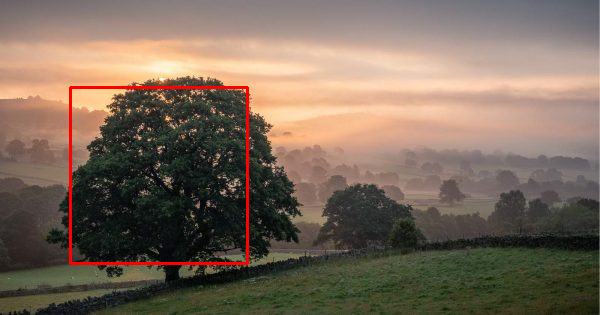
\includegraphics[width=.9\textwidth]{images/results/6fin}
\end{figure}
$N_{superpixel}=750$, $N=1$. The tree is not correctly localized, the right part is not corrected classified. When a very few of superpixel are classified correctly, increasing $N$ can help a lot.
\newpage

\subsection{Result on test 7}
\begin{figure}[htpb] 
	\centering
	\begin{minipage}{.3\textwidth}
		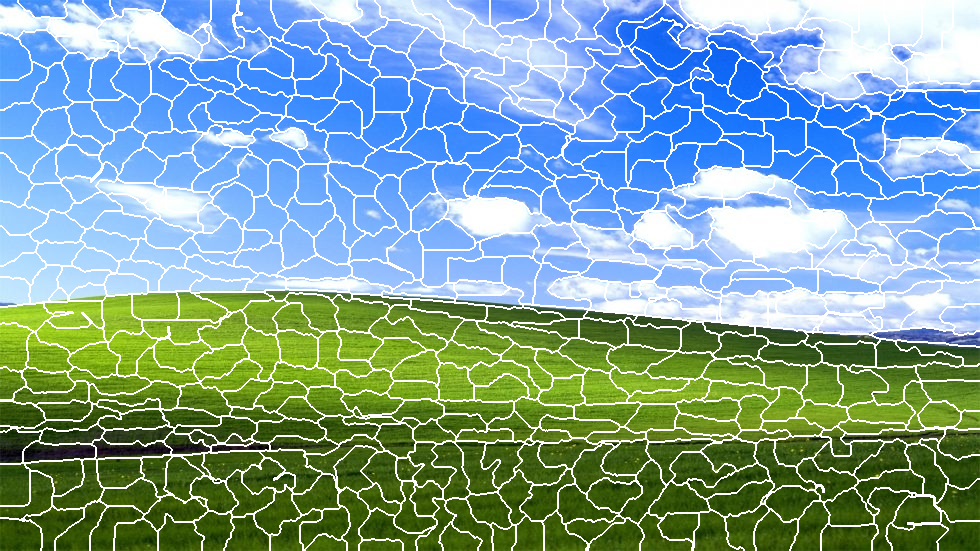
\includegraphics[width=1.7\textwidth]{images/results/7seg} 
	\end{minipage}
	\hspace{.25\textwidth}
	\begin{minipage}{.3\textwidth}
		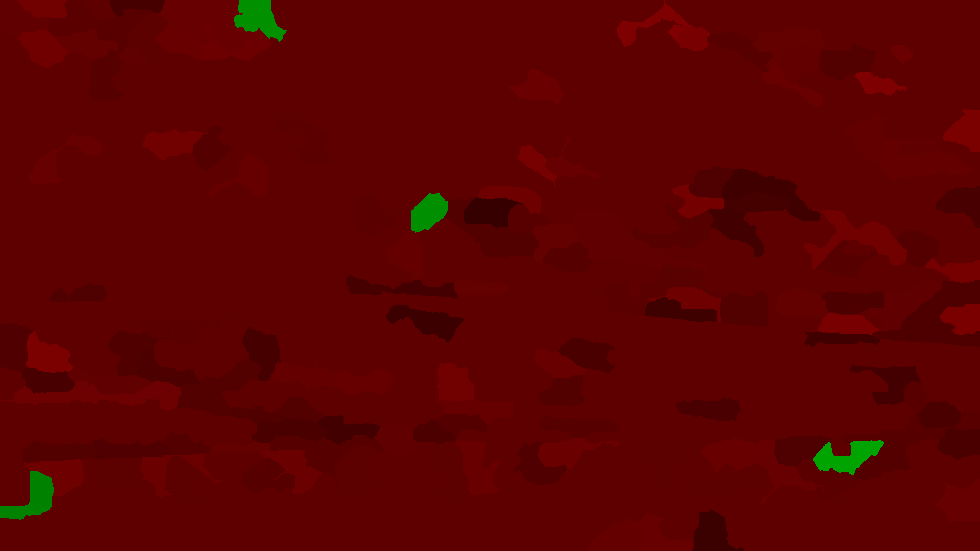
\includegraphics[width=1.7\textwidth]{images/results/7map}
	\end{minipage}  
\end{figure}
\begin{figure}[htpb]
	\centering
	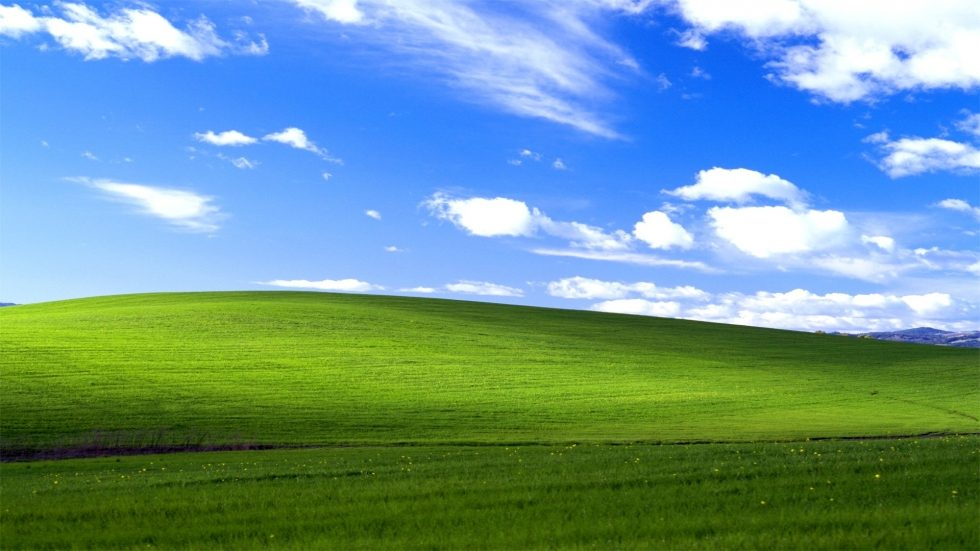
\includegraphics[width=.9\textwidth]{images/results/7fin}
\end{figure}
$N_{superpixel}=750$, $N=0$. Everything seems working here. Three superpixels are classified correctly but they're too small to be considered as a tree.
\newpage

\subsection{Result on test 8}
\begin{figure}[htpb] 
	\centering
	\begin{minipage}{.3\textwidth}
		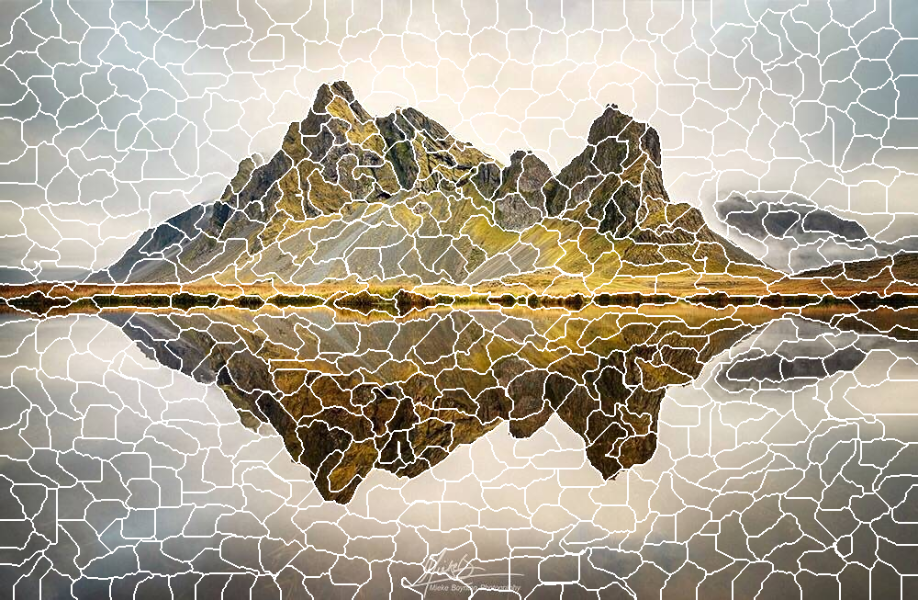
\includegraphics[width=1.7\textwidth]{images/results/8seg} 
	\end{minipage}
	\hspace{.25\textwidth}
	\begin{minipage}{.3\textwidth}
		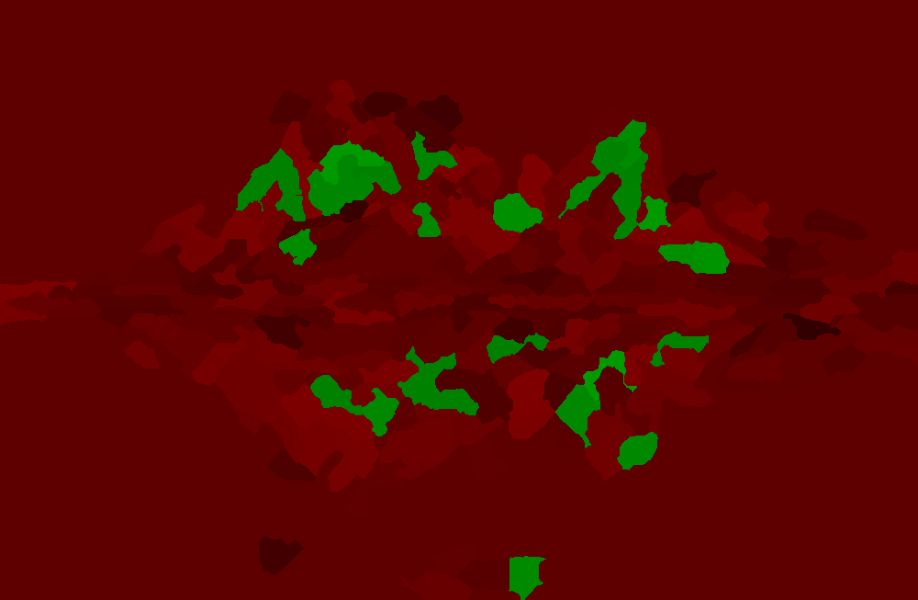
\includegraphics[width=1.7\textwidth]{images/results/8map}
	\end{minipage}  
\end{figure}
\begin{figure}[htpb]
	\centering
	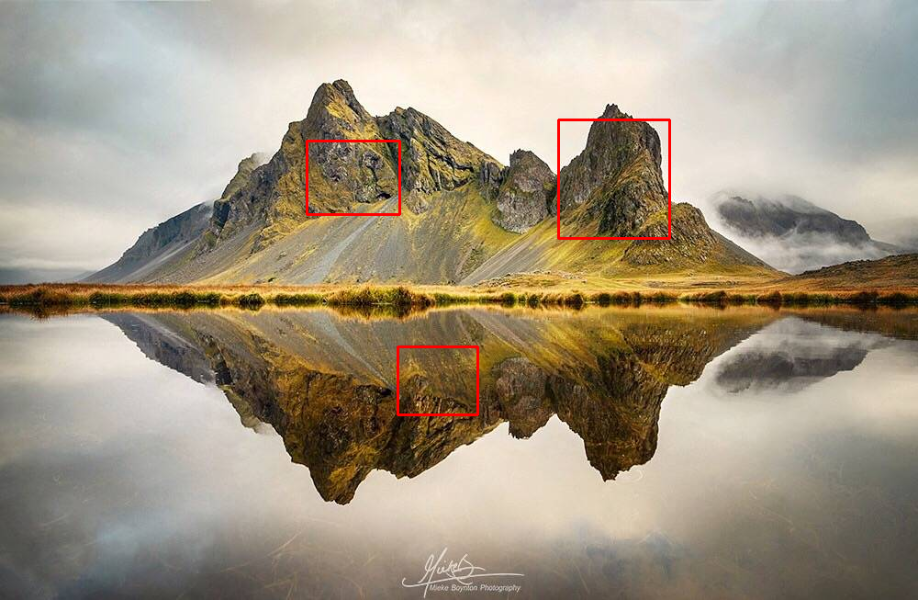
\includegraphics[width=.9\textwidth]{images/results/8fin}
\end{figure}
$N_{superpixel}=750$, $N=0$. There are three false positive that can be discarded by color thresholding. A more robust SVM will cancel out the problem without that.
\newpage

\subsection{Result on test 9}
\begin{figure}[htpb] 
	\centering
	\begin{minipage}{.3\textwidth}
		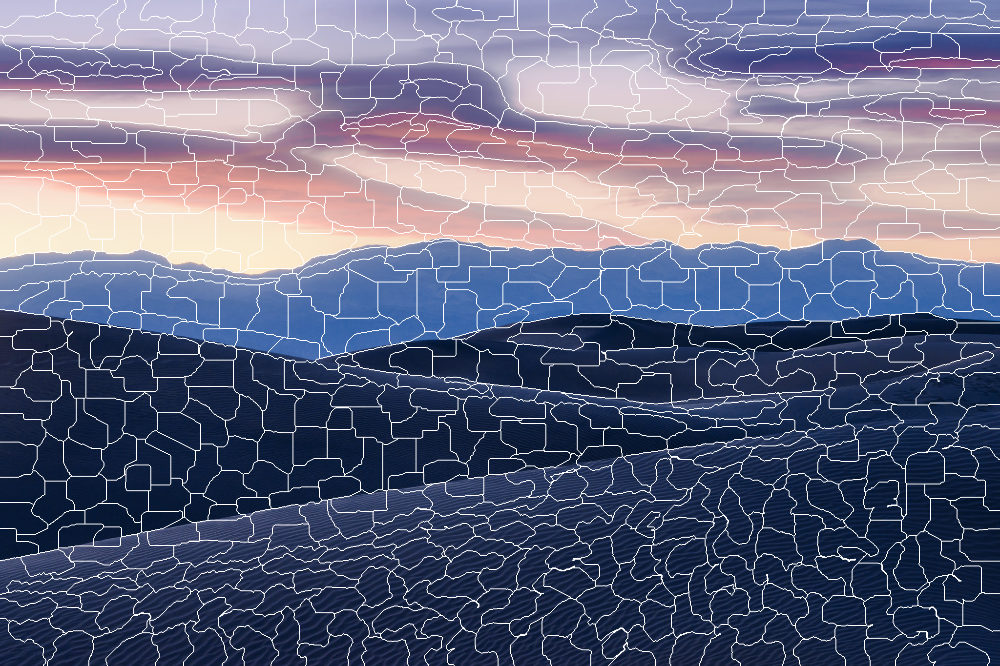
\includegraphics[width=1.7\textwidth]{images/results/9seg} 
	\end{minipage}
	\hspace{.25\textwidth}
	\begin{minipage}{.3\textwidth}
		
\includegraphics[width=1.7\textwidth]{images/results/9map}
	\end{minipage}  
\end{figure}
\begin{figure}[htpb]
	\centering
	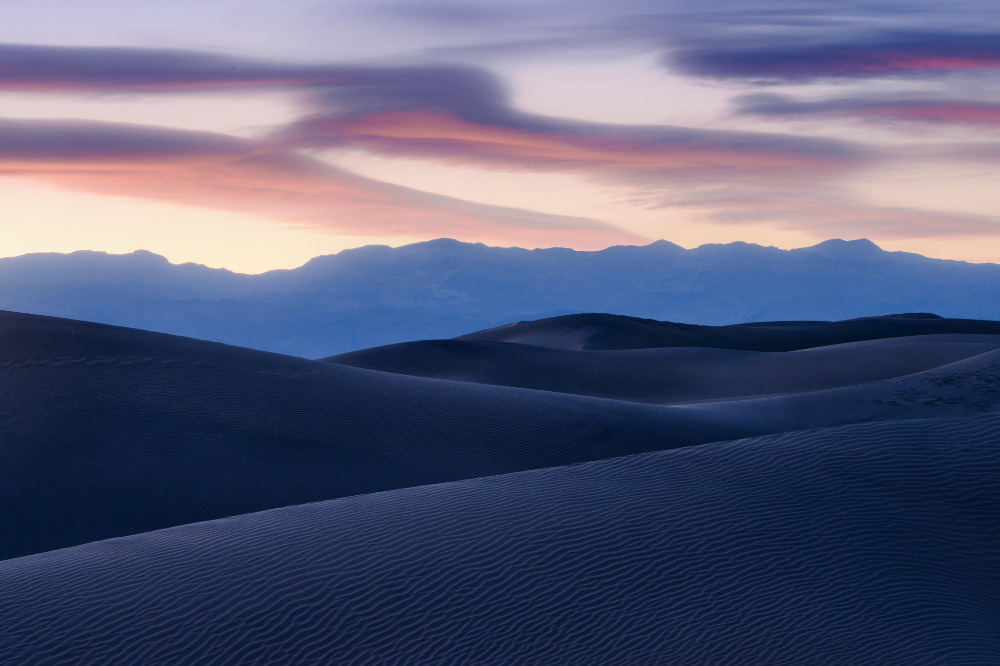
\includegraphics[width=.9\textwidth]{images/results/9fin}
\end{figure}
$N_{superpixel}=750$, $N=0$. Everything works here. The low classification probabilities are due to the very few features.
\newpage

\subsection{Result on test 10}
\begin{figure}[htpb] 
	\centering
	\begin{minipage}{.3\textwidth}
		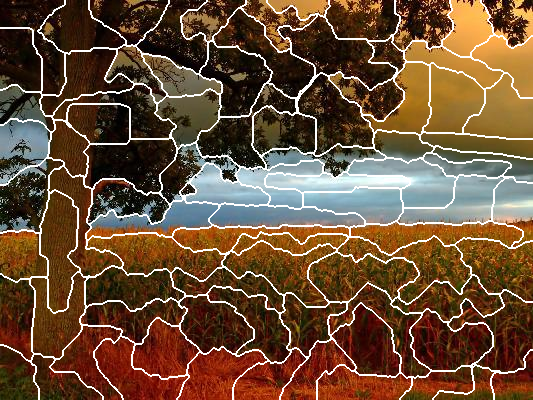
\includegraphics[width=1.7\textwidth]{images/results/10seg} 
	\end{minipage}
	\hspace{.25\textwidth}
	\begin{minipage}{.3\textwidth}
		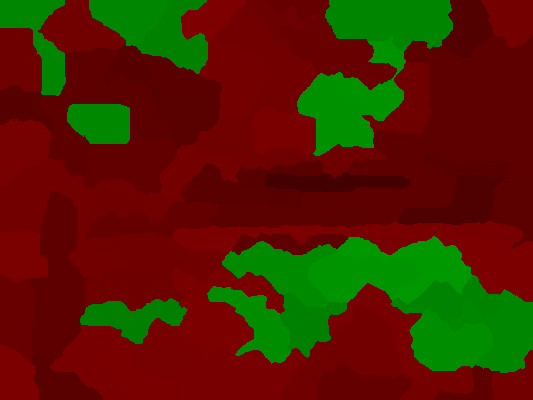
\includegraphics[width=1.7\textwidth]{images/results/10map}
	\end{minipage}  
\end{figure}
\begin{figure}[htpb]
	\centering
	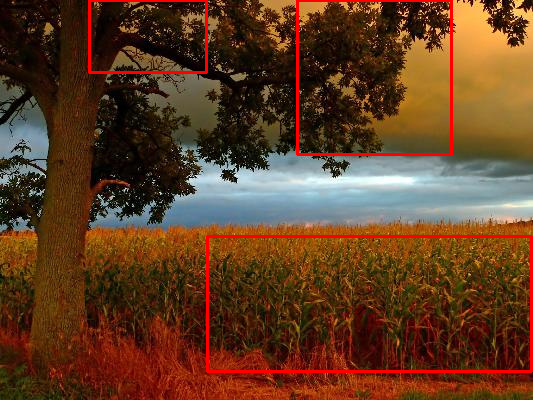
\includegraphics[width=.9\textwidth]{images/results/10fin}
\end{figure}
$N_{superpixel}=150$, $N=0$. There's a false positive. The other two bounding boxes are not connected.
\newpage

\subsection{Result on test 11}
\begin{figure}[htpb] 
	\centering
	\begin{minipage}{.3\textwidth}
		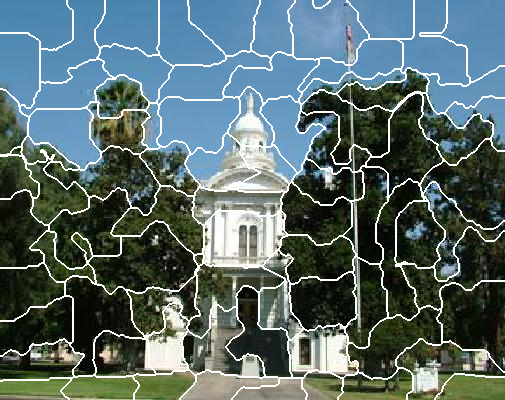
\includegraphics[width=1.7\textwidth]{images/results/11seg} 
	\end{minipage}
	\hspace{.25\textwidth}
	\begin{minipage}{.3\textwidth}
		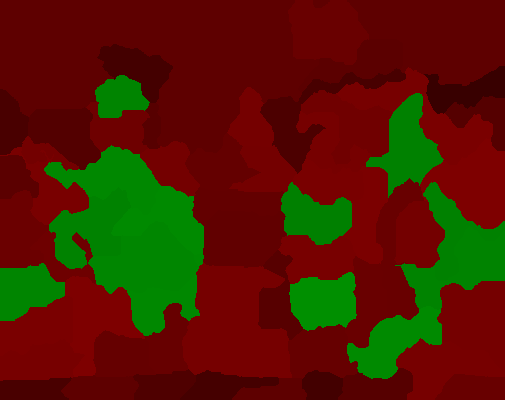
\includegraphics[width=1.7\textwidth]{images/results/11map}
	\end{minipage}  
\end{figure}
\begin{figure}[htpb]
	\centering
	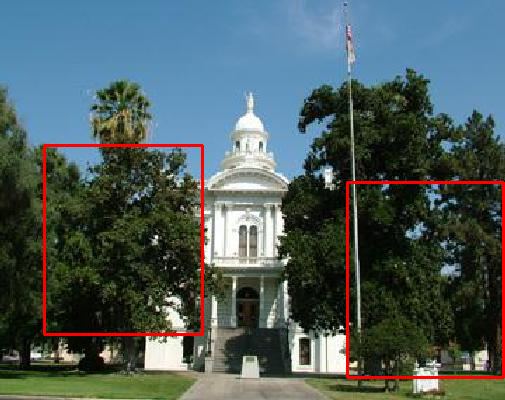
\includegraphics[width=.9\textwidth]{images/results/11fin}
\end{figure}
$N_{superpixel}=150$, $N=0$. The left tree is nicely localized. The right tree no. I choose to present this image because there's a pole in the middle, histogram aggregation can avoid this problem (but in this particular case it doesen't work) 

\newpage
\subsection{Result on test 12}
\begin{figure}[htpb] 
	\centering
	\begin{minipage}{.3\textwidth}
		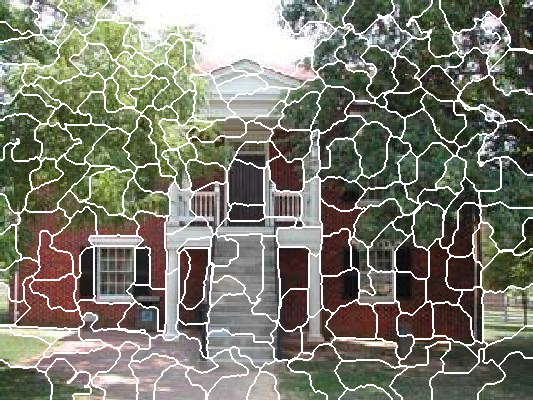
\includegraphics[width=1.7\textwidth]{images/results/12seg} 
	\end{minipage}
	\hspace{.25\textwidth}
	\begin{minipage}{.3\textwidth}
		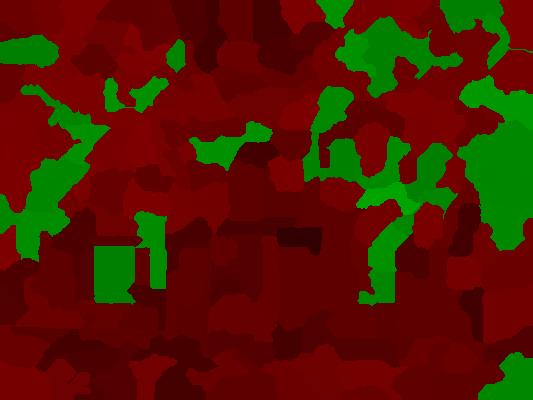
\includegraphics[width=1.7\textwidth]{images/results/12map}
	\end{minipage}  
\end{figure}
\begin{figure}[htpb]
	\centering
	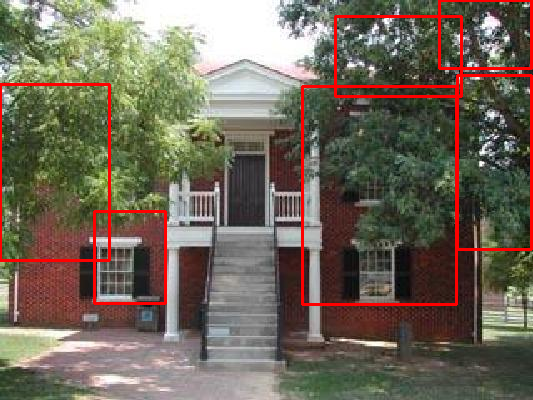
\includegraphics[width=.9\textwidth]{images/results/12fin}
\end{figure}
$N_{superpixel}=450$, $N=0$. The right tree shows a weak connectivity, that can be avoided not by aggregating on HSV color space but instead on spatiality.





\end{document}
